\large
%%ANC headphones are becoming widely used in consumer electronics, however often the attenuation decreases rapidly with an increased frequency. 
%%This is due to the delays introduced by sampling and reconstructing the signals.
%This can be due to delay in the ANC system. 
%A Linear Prediction (LP) algorithm is proposed to predict $P$ samples, corresponding to the system delay, to compensate for the delay.   
%\begin{centering}
%	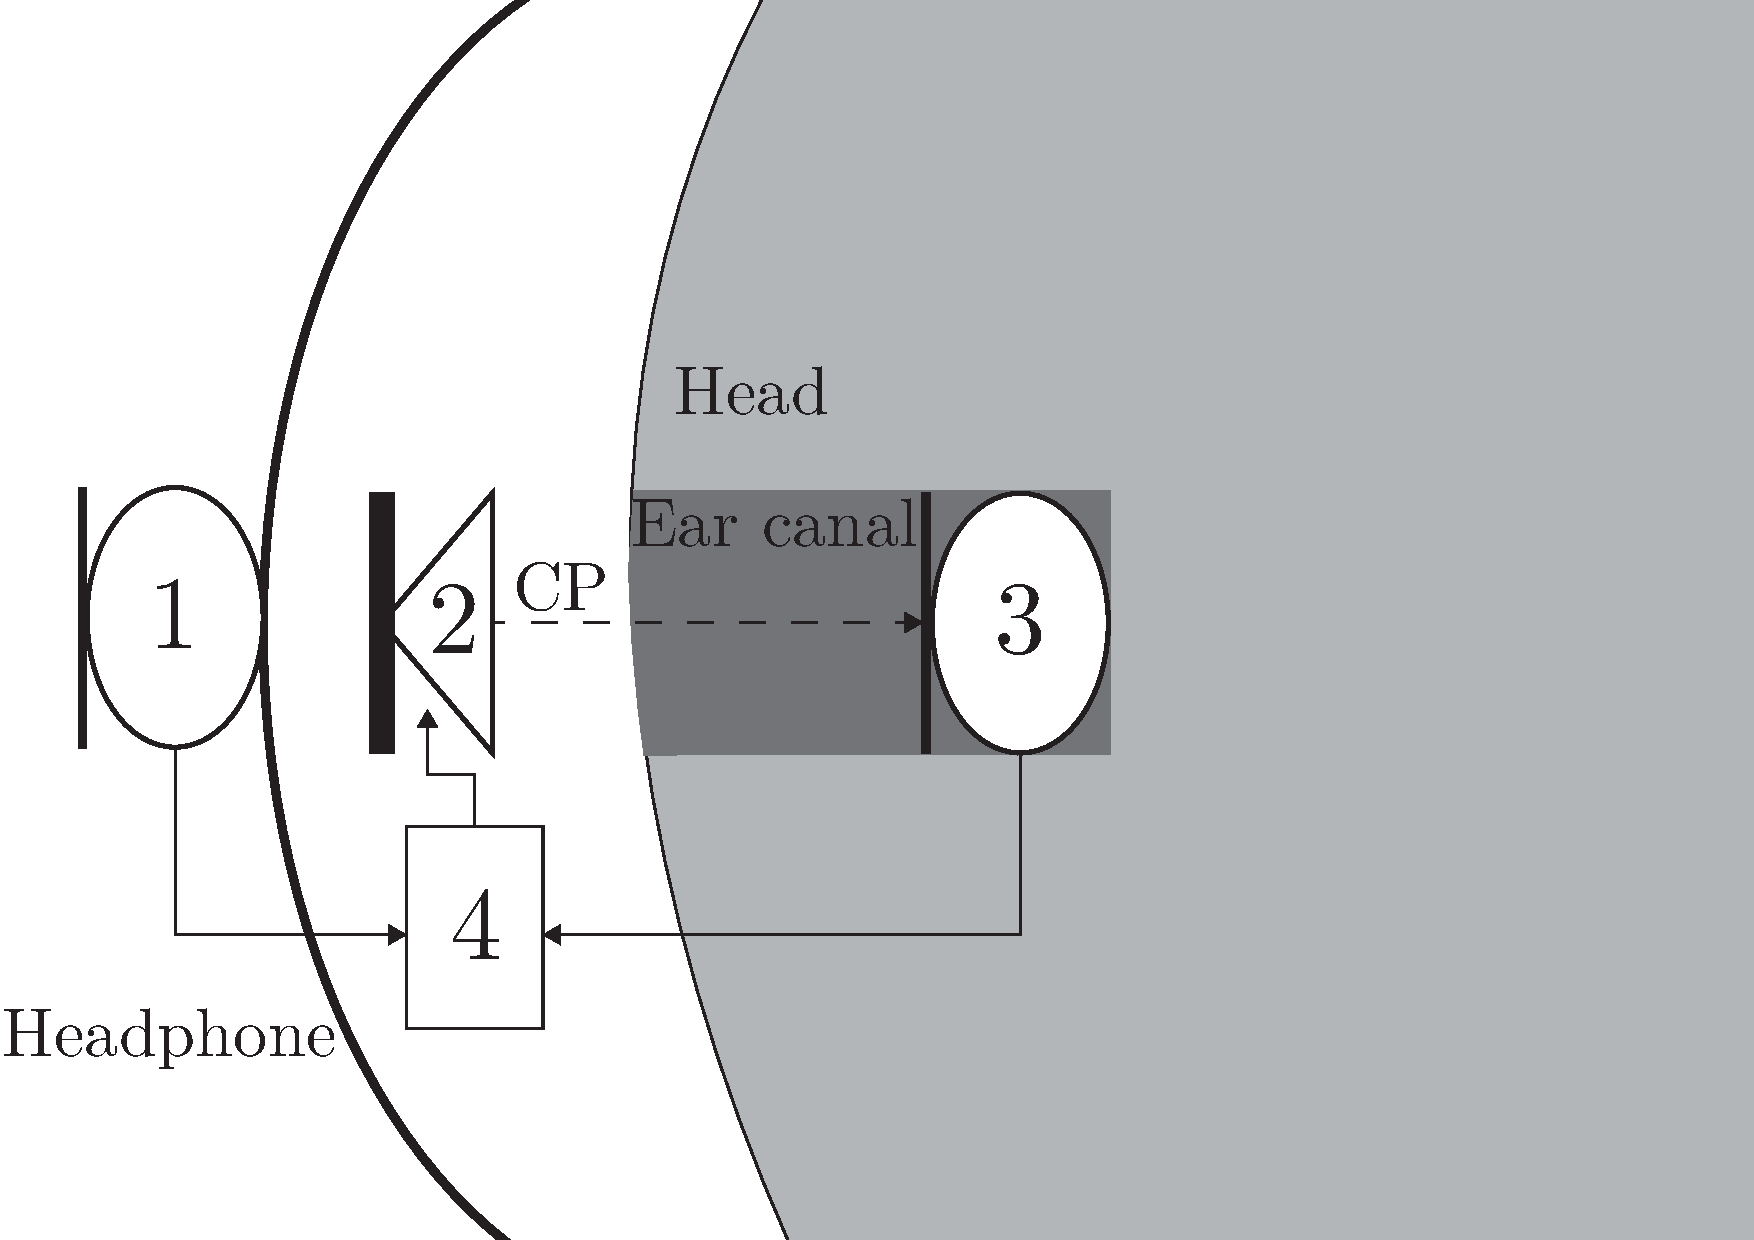
\includegraphics[width=\textwidth]{figures/BasicOverviewZoomed.pdf}
%\end{centering}
%The simulated test setup consists of a reference microphone (1), a headphone speaker (2), an error microphone (3) and a DSP (4). %The delays are introduced by sampling the microphones and playing the counterphase signal through the loudspeaker.\\ 

%
%
%
%%Oliver Edition
%% % ANC headphones are becoming increasingly popular, especially for canceling speech. 
% In order to cancel speech, a feedforward solution is proposed.
% However this method introduces increasingly large delay, and to accommodate this problem, a Linear Prediction (LP) algorithm is proposed to predict $P$ samples
% of the speech signal, thus compensating for the delay.
%
%
%\begin{centering}
%	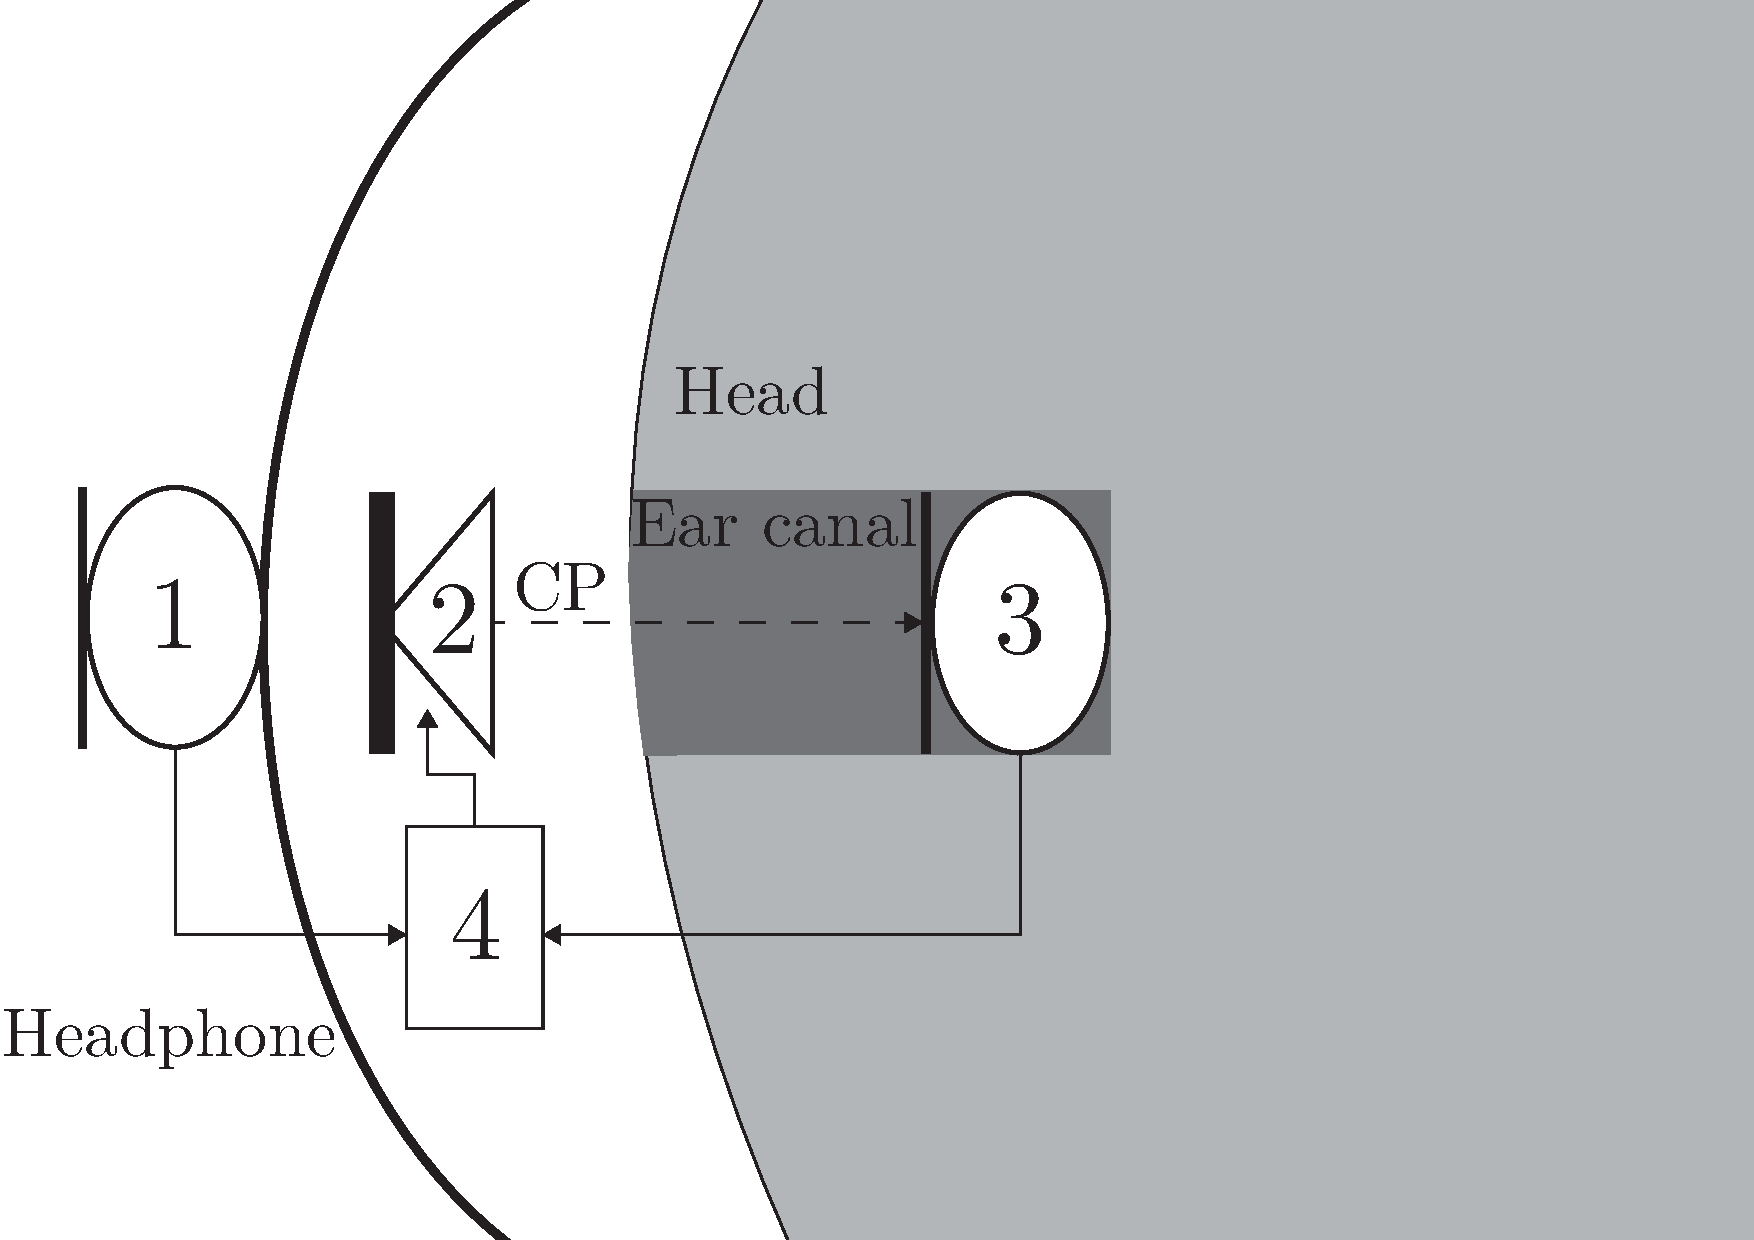
\includegraphics[width=\textwidth]{figures/BasicOverviewZoomed.pdf}
%\end{centering}
%The simulated test setup consists of a reference microphone (1), a headphone speaker (2), an error microphone (3) and a DSP (4). 
%
%speech
%feedforward
%delay
%LP


%ANC headphones are used to attenuate various noise sources, among these are speech.


%Active Noise Control (ANC) headphones lack the ability to attenuate speech.
%In order to remedy this problem, a feedforward system is necessary.
%This feedforward topology introduces delay, which decreases the attenuation of the system.
%In order to compensate for delay, a Linear Prediction (LP) scheme is proposed.



% C verison:
Active Noise Control (ANC) headphones have limited speech attenuation.
When using a digital solution, delays are introduced, which decreases attenuation. This can be remedied using Linear Prediction (LP).
\vspace{-7mm}
\resizebox{1\columnwidth}{!}{
\begin{tikzpicture}
\draw [](-2.92,2.32) node (v1) {} .. controls (-3.26,2.06) and (-3.26,0.54) .. (-2.92,0.32) node (v2) {};

\draw [draw=black,fill=black!20](-0.68,2.32) node (v1) {} .. controls (-1.08,2.06) and (-1.08,0.54) .. (-0.68,0.32) node (v2) {};
\draw [white, fill=black!20](-0.68,2.32) -- (1.56,2.32) -- (1.56,0.32) -- (-0.68,0.32);


\draw [draw=black,fill=black!60](-0.93,1.78) node (v1) {} .. controls (-0.99,1.59) and (-0.99,1.14) .. (-0.95,0.94) node (v2) {};
\draw [draw=black,fill=black!60](-0.93,1.78) -- (0.72,1.78) -- (0.72,0.94) -- (-0.95,0.94);


\draw [draw=black,fill=white] (0.48,1.36) node (v3) {3} ellipse (0.2 and 0.3);
\draw [draw=black,fill=black](0.28,1.66) -- (0.28,1.06);

\draw [draw=black,fill=white] (-3.4,1.36) node (v3) {1} ellipse (0.2 and 0.3);
\draw [draw=black,fill=black](-3.6,1.7) -- (-3.6,1.06);


\draw [draw=black,fill=black] (-2.9,1.7) rectangle (-3,1);
\draw (-2.9,1.3) -- (-2.6,1.7) -- (-2.6,1) -- (-2.9,1.3);
\node at (-2.7,1.34) {\small{2}};


\draw[->,dashed] (-2.6,1.36) node[right=16.5,above=2]{\small{CP}}-- (0.28,1.36);
\draw[fill=black!20]  (-2.1,0.82) rectangle node{4}(-2.5,0.36);
\draw [<-](-2.5,0.54) -- (-3.4,0.54) -- (-3.4,1.06);
\draw [<-](-2.1,0.54) -- (0.48,0.54) -- (0.48,1.06);
\draw [->](-2.3,0.82) -- (-2.3,0.86) -- (-2.94,0.86) -- (-2.94,1);
\node at (0,2) {\small{Ear Canal}};
\node[anchor=south west,inner sep=0] at (1.9,0.3) {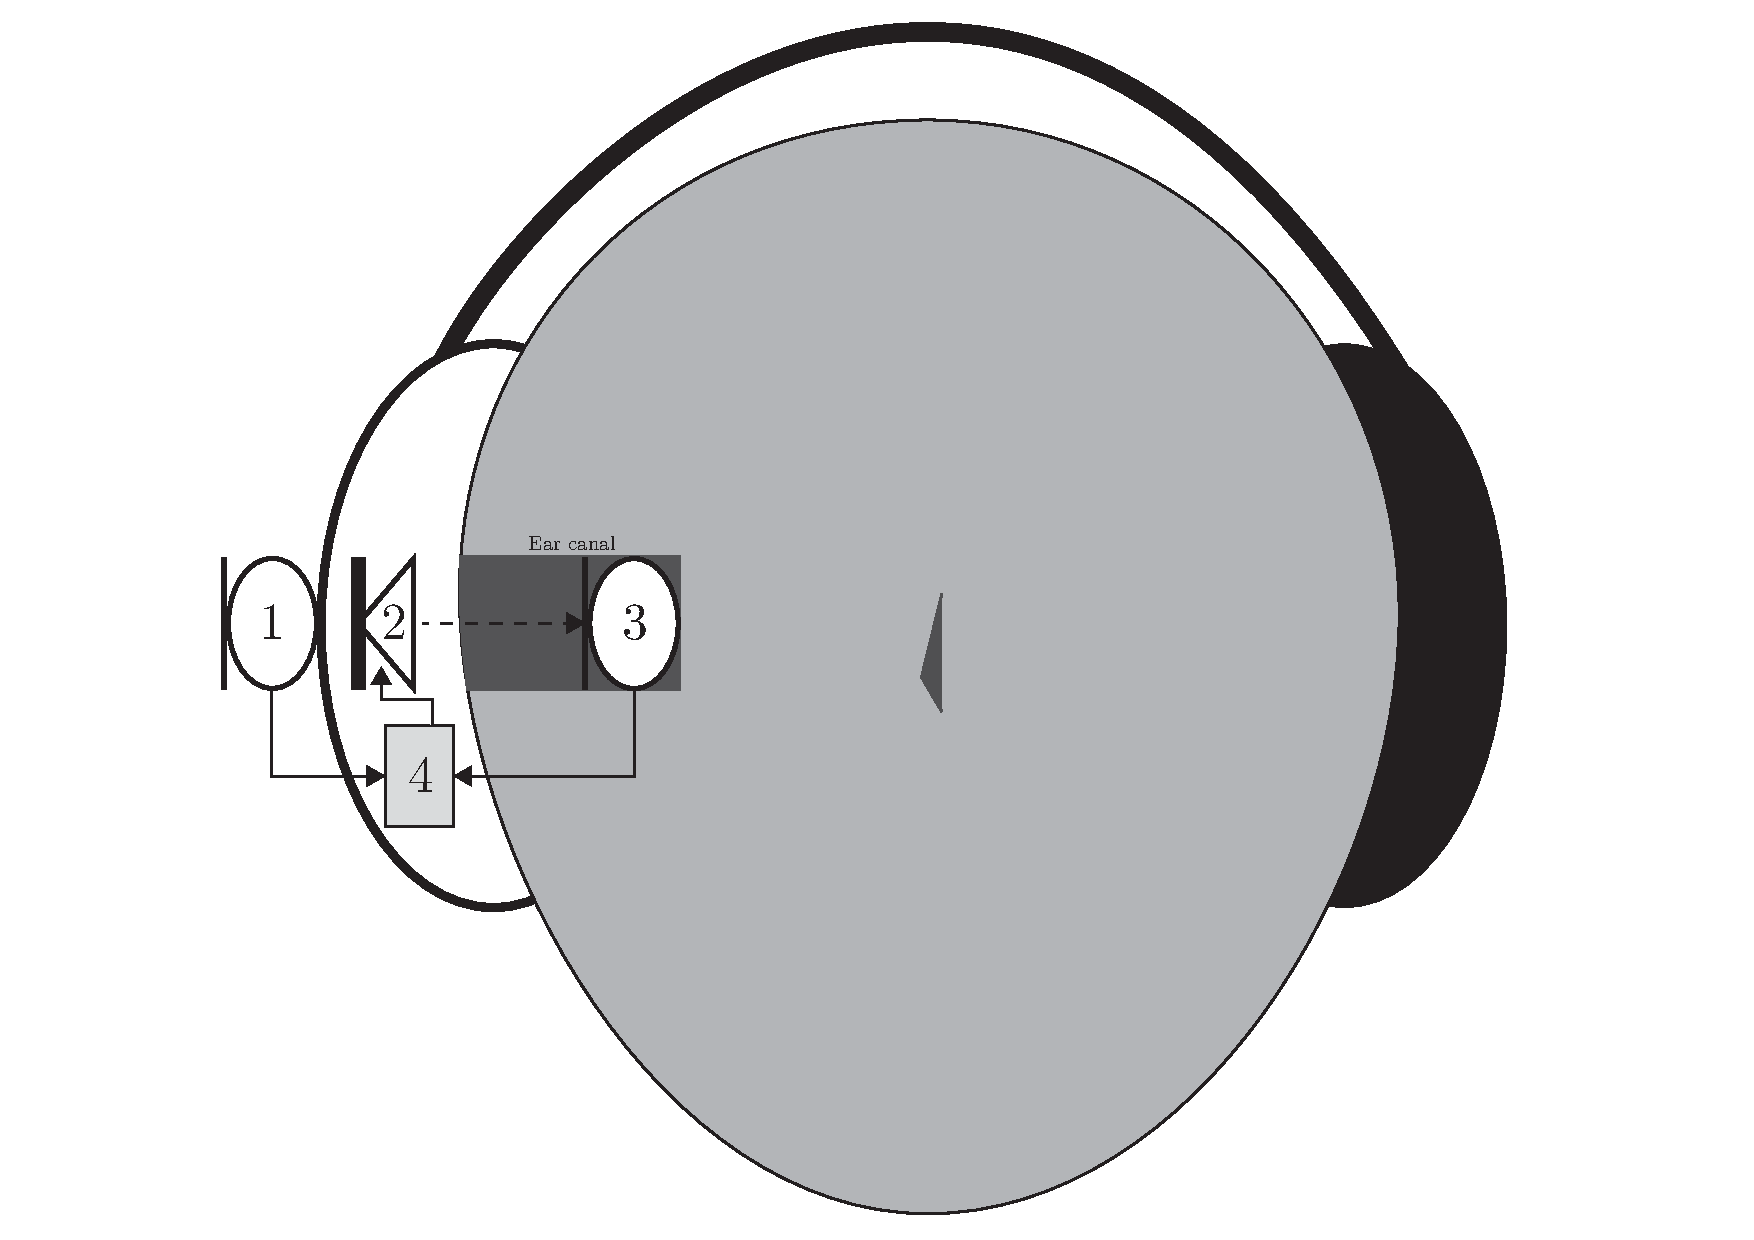
\includegraphics[width=3cm]{BasicOverview}};

\draw  (3.14,1.65) rectangle (2.14,0.95);

\draw (1.56,1.31) -- (2.14,1.31);
\draw  (1.56,2.32) rectangle (-3.7,0.32);
\end{tikzpicture}
}

\vspace{6mm}
The simulated feedforward test setup consists of a reference microphone (1), a headphone speaker (2), an error microphone (3) and a DSP (4).



 











